\chapter{Artificial Neural Networks}\label{chp:3}

We saw in section \ref{limitations}, that the practical applicability of linear models with fixed basis functions is limited. One alternative is choosing a fixed number of \textcolor{blue}{\emph{adaptive basis functions}}. Here, basis functions are parametrized in a suitable way, and the parameters are adapted during the training in such a way such that the model explains (or “tuned” to) the given data. This approach can be carried out via using \textcolor{blue}{\emph{artificial neural networks}}, which we define in what follows.

\section{Fundamental Aspects}

\begin{definition}[Artificial Neural Network]
For a fixed $L \in \mathbb{N}$, let $n_0, \dots, n_L \in \mathbb{N}, W^{[\ell]} \in \mathbb{R}^{n_{\ell} \times n_{\ell -1}},$ and $b^{[\ell]} \in \mathbb{R}^{n_{\ell}}$ for all $\ell = 1, \dots, L$. Furthermore, let $g^{[\ell]}: \mathbb{R}^{n_{\ell}} \rightarrow \mathbb{R}^{n_{\ell}}$ for $\ell = 1, \dots, L$ be some functions. Then the function $f_{\theta} : \mathbb{R}^{n_0} \rightarrow \mathbb{R}^{n_L}$, which maps an \textcolor{blue}{\emph{input vector}} $x \in \mathbb{R}^{n_0}$ to
\begin{align}
    &f_{\theta}(x) := a^{[L]}, \quad \text{where}\\
    &a^{[0]} := x,\\
    &z^{[\ell]} := W^{[\ell]} a^{[\ell-1]} + b^{[\ell]},\\
    &a^{[\ell]} := g^{[\ell]}(z^{[\ell]}), \Biggr\} \quad \ell = 1, \ldots, L
    \label{eqn:29}
\end{align}

is called an \textcolor{blue}{\emph{artificial neural network}} with \textcolor{blue}{\emph{parameters}} $\theta = (W^{[1]}, b^{[1]}, \ldots, W^{[L]}, b^{[L]})$ and \textcolor{blue}{\emph{activation functions}} $g^{[1]}, \ldots, g^{[L]}$. The matrices $W^{[1]}, \ldots, W^{[L]}$ are called \textcolor{blue}{\emph{weight matrices}}, and the vectors $b^{[1]}, \ldots, b^{[L]}$ are called \textcolor{blue}{\emph{bias vectors}} of $f$.\\

For fixed $x \in \mathbb{R}^n_0$ and $\ell \in \{1, \ldots, L\}$, we call $z^{[\ell]} \in \mathbb{R}^{n_{\ell}}$ \textcolor{blue}{\emph{(net) input vector)}} and $a^{[\ell]} \in \mathbb{R}^{n_{\ell}}$ the \textcolor{blue}{\emph{activation vector)}} in the $\ell$-th layer, where $n_{\ell}$ is the \textcolor{blue}{\emph{width)}} of the $\ell$-th layer. Finally, $f_{\theta}(x)=a^{[L]}$ is the \textcolor{blue}{\emph{output vector)}}, and $L$ is called the \textcolor{blue}{\emph{depth)}} of $f_{\theta}$.
\end{definition}

\begin{figure}[h!]
    \centering
    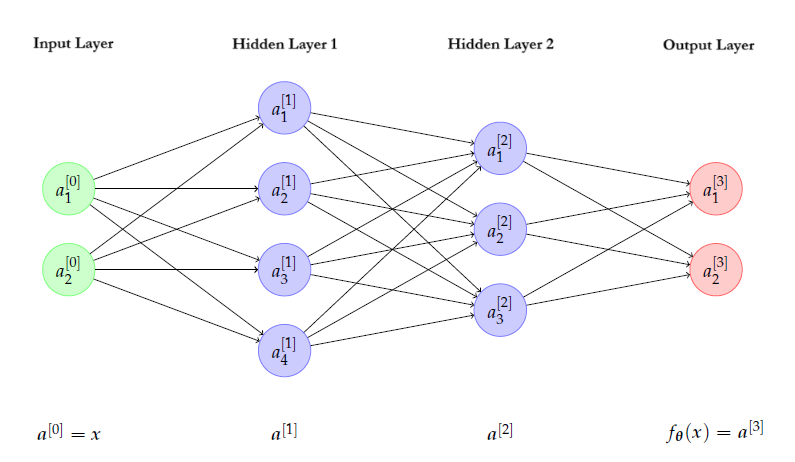
\includegraphics[width=\textwidth]{images/figure6.png}
    \caption{Example of an artificial neural network with two hidden layers.}
    \label{fig:6}
\end{figure}

\begin{remark}[Nonlinearity]
The vectors $a^{[0]}, \ldots, a^{[L]}$ and $z^{[1]}, \ldots, z^{[L]}$ defined in \ref{eqn:29} are, like $f_{\theta}$, functions of the input vector $x$. For simplicity, we usually omit this dependency in our notation as long as the context is clear. Nevertheless, we can understand $f_{\theta}$ as a composition of several linear and nonlinear functions. For example, for $L=1$ we have

\begin{equation}
    f_{\theta}(x) = g^{[1]}(W^{[1]}x + b^{[1]}),
    \label{eqn:30}
\end{equation}\\

meaning that $f_{\theta}$ is a composition of $g^{[1]}$ with $z^{[1]} = W^{[1]}x + b^{[1]}$. Also for $L=2$ we obtain a function

\begin{equation}
    f_{\theta}(x) = g^{[2]}(W^{[2]}(g^{[1]}(W^{[1]}x + b^{[1]})) + b^{[2]}),
    \label{eqn:31}
\end{equation}\\
and the process continues in the same way for $L \geq 3$.\\

In general at least some of the functions $g^{[\ell]}$ are chosen to be nonlinear. If this was not the case, then $f_{\theta}$, as a composition of linear functions, would also be linear. The additional and more complex structure \ref{eqn:29} would therefore have no advantage over a simple representation of the form $f_{\theta}(x) = Wx + b$ with $W \in \mathbb{R}^{n_L \times n_0}$ and $b \in \mathbb{R}^{n_L}$ (as every affine-linear function can be represented in such a way).

\end{remark}

\begin{remark}[Scalar Activation Functions]
The activation function $g^{[\ell]}: \mathbb{R}^{n_{\ell}} \rightarrow \mathbb{R}^{n_{\ell}}$ can often be interpreted as a component-wise application of a real function from $\mathbb{R}$ to $\mathbb{R}$. In this case, unless stated differently, for a scalar function $g^{[\ell]}: \mathbb{R} \rightarrow \mathbb{R}$, we define $g^{[\ell]}(z) \in \mathbb{R}^{n_{\ell}}$ as a component-wise application of $g^{[\ell]}$ to $z \in \mathbb{R}^{n_{\ell}}$,

\begin{equation}
    g^{[\ell]}(z) := \begin{pmatrix}
    g^{[\ell]}(z_1) \\
    \vdots \\
    g^{[\ell]}(z_{n_\ell})
    \end{pmatrix}.
    \label{eqn:32}
\end{equation}

\end{remark}

When defining a neural network, we decide on the type of activation functions that we use.
Below we give a few example of commonly used activation functions.

\begin{example}[Typical Activation Functions]
Depending on the context and goal of the problem, we can use any of the below activation functions (see Figure \ref{fig:7}) while defining the neural network:

\begin{figure}[h!]
    \centering
    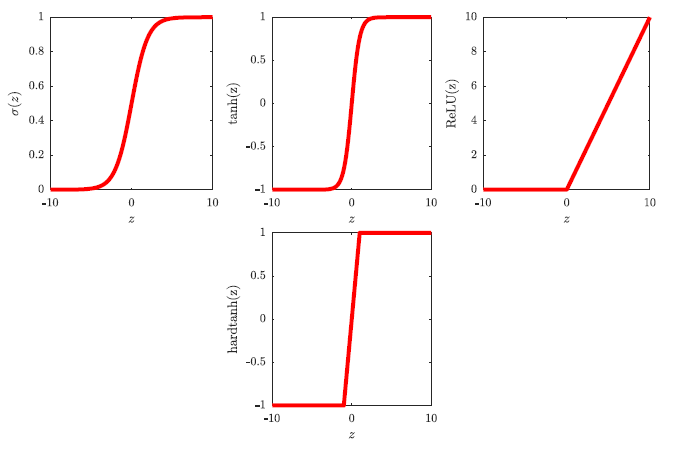
\includegraphics[width=0.8\textwidth]{images/figure7.png}
    \caption{Typical Activation Functions}
    \label{fig:7}
\end{figure}

\begin{itemize}
    \item \textcolor{blue}{\emph{Sigmoid function}}: Commonly used in the output layer of a binary classification task, as it maps values to the range $(0, 1)$, representing probabilities. Suitable when the model needs to output probabilities or interpret values as likelihoods, but it can suffer from vanishing gradients.\cite{hochreiter1997lstm, rumelhart1986learning}
    \begin{equation}
        \sigma: \mathbb{R} \to (0,1), \quad \sigma(z) := \frac{1}{1+e^{-z}}
        \label{eqn:33}
    \end{equation}
    
    \item \textcolor{blue}{\emph{ReLU (Rectified Linear Unit) function}}: It ensures sparsity by retaining only positive activations, which not only introduces non-linearity but also improves computational efficiency and helps avoid the vanishing gradient problem.\cite{nair2010relu}
    \begin{equation}
        \text{ReLU}(z): \mathbb{R} \to \mathbb{R}_{\geq 0}, \quad \text{ReLU}(z) := \max(0, z)
        \label{eqn:34}
    \end{equation}
    
    \item \textcolor{blue}{\emph{Hyperbolic Tangent (tanh) function}}: Preferred in hidden layers when inputs are zero-centered, as it maps the input in the range $(-1, 1)$, which helps faster convergence during training. It has more efficient gradient flow than sigmoid function.
    \begin{equation}
        \text{tanh}: \mathbb{R} \to (-1,1), \quad \text{tanh}(z) := \frac{e^z-e^{-z}}{e^z+e^{-z}}
        \label{eqn:35}
    \end{equation}
    
    \item \textcolor{blue}{\emph{Hard hyperbolic tangent (hardtanh) function}}: Provides a faster approximation of the traditional tanh function, maintaining a balance between non-linearity and computational simplicity.
    \begin{equation}
        \text{hardtanh}(z): \mathbb{R} \to [-1,1], \quad \text{hardtanh}(z) := \max(-1, \min(1,z))
        \label{eqn:36}
    \end{equation}
    
    \item \textcolor{blue}{\emph{Identity function}}: While it does not introduce non-linearity, it is occasionally used in skip connections or output layers when no transformation is needed.
    \begin{equation}
        \text{id}(z): \mathbb{R} \to \mathbb{R}, \quad \text{id}(z) := z
        \label{eqn:37}
    \end{equation}
    
    \item \textcolor{blue}{\emph{Softmax function}}: Typically applied at the output layer for multi-class classification tasks, converting raw scores into normalized probabilities.
    \begin{equation}
        \text{softmax}(z) : \mathbb{R}^n \to \mathbb{R}^n, \quad \text{softmax}(z)_j := \frac{e^{z_j}}{\sum_{j=1}^n e^{z_j}}
        \label{eqn:38}
    \end{equation}
\end{itemize}

\end{example}

\section{Multiclass Classification}

\vspace{5em}
\textbf{TO BE CONTINUED...}


